\documentclass[runningheads]{llncs}
\usepackage{amssymb}
\setcounter{tocdepth}{3}
\usepackage{graphicx,epsfig}
\usepackage{algorithmic}
\usepackage{listings}
\usepackage{rotating}
\usepackage{subfig}
\usepackage{listings}
\usepackage{wrapfig}
%%%%

\usepackage{color}
\usepackage{alltt}
\usepackage{verbatim}
\usepackage{url}
\usepackage[utf8]{inputenc}
\usepackage[spanish,es-noshorthands]{babel}

%%

\usepackage{url}

% Style definition file generated by highlight 2.9, http://www.andre-simon.de/ 

% Highlighting theme definition: 

\newcommand{\hlstd}[1]{\textcolor[rgb]{0,0,0}{#1}}
\newcommand{\hlnum}[1]{\textcolor[rgb]{0.5,0,0.5}{\bf{#1}}}
\newcommand{\hlesc}[1]{\textcolor[rgb]{1,0,1}{\bf{#1}}}
\newcommand{\hlstr}[1]{\textcolor[rgb]{0.65,0.52,0}{#1}}
\newcommand{\hlpps}[1]{\textcolor[rgb]{0,0,1}{#1}}
\newcommand{\hlslc}[1]{\textcolor[rgb]{0.95,0.47,0}{#1}}
\newcommand{\hlcom}[1]{\textcolor[rgb]{1,0.5,0}{#1}}
\newcommand{\hlppc}[1]{\textcolor[rgb]{0,0.5,0.75}{\bf{#1}}}
\newcommand{\hlopt}[1]{\textcolor[rgb]{1,0,0.5}{\bf{#1}}}
\newcommand{\hlipl}[1]{\textcolor[rgb]{0.62,0.36,1}{#1}}
\newcommand{\hllin}[1]{\textcolor[rgb]{0.19,0.19,0.19}{#1}}
\newcommand{\hlkwa}[1]{\textcolor[rgb]{0.73,0.47,0.47}{\bf{#1}}}
\newcommand{\hlkwb}[1]{\textcolor[rgb]{0.5,0.5,0.75}{\bf{#1}}}
\newcommand{\hlkwc}[1]{\textcolor[rgb]{0,0.5,0.75}{#1}}
\newcommand{\hlkwd}[1]{\textcolor[rgb]{0,0.27,0.4}{#1}}
\definecolor{bgcolor}{rgb}{0.93,0.93,0.93}

%\urldef{\mailsa}\path|pgarcia@atc.ugr.es|

\urldef{\mailsa}\path|pgarcia@atc.ugr.es|

\newcommand{\keywords}[1]{\par\addvspace\baselineskip
\noindent\keywordname\enspace\ignorespaces#1}

\lstset{
basicstyle=\ttfamily \scriptsize,
language=c++,
frame=single,
stringstyle=\ttfamily,
showstringspaces=false
}

\renewcommand{\textfraction}{0}
\renewcommand{\topfraction}{1}
\renewcommand{\bottomfraction}{1}
\renewcommand{\floatpagefraction}{0.9}

\begin{document}

\mainmatter  % start of an individual contribution



% first the title is needed
\title{Desarrollo de servicios para una Arquitectura Orientada a Servicios para Algoritmos Evolutivos}
% Muchos servicios me parecen ¿Resolviendo problemas? ¿Creando aplicaciones? ¿Desarrollo ágil? - JJ - FERGU: es que se desarrollan varios


% a short form should be given in case it is too long for the running head
\titlerunning{Desarrollo de servicios para una SOA para EAs}
%\author{No author given}
\author{P. García-Sánchez, M. García-Arenas, A. M. Mora, P.A. Castillo, C. Fernandes, J. González, G. Romero, J.J. Merelo y P. de Las Cuevas}

%

%\authorrunning{P. Garc\'ia-S\'anchez et al.}
%\authorrunning{Anonymous.}
% (feature abused for this document to repeat the title also on left hand pages)
% the affiliations are given next; don't give your e-mail address
% unless you accept that it will be published

\institute{Dept. de Arquitectura y Tecnología de Computadores, Universidad de Granada \and LaSEEB-ISR-IST, Technical University of Lisbon (IST), Lisboa, Portugal
\mailsa}
%\institute{No institute given
%\mailsa}




%\toctitle{BLABLABLA}

%\tocauthor{Authors' Instructions}
\maketitle
\thispagestyle{empty}
\pagestyle{empty}
\begin{abstract}
Este artículo muestra el diseño e implementación de servicios para
Computación Evolutiva dentro del paradigma de la Arquitectura
Orientada a Servicios. Este paradigma proporciona independencia en el
lenguaje y comunicación, pero el desarrollo requiere tratar con
algunas cuestiones tecnológicas y de diseño, como un diseño lo más
abstracto posible o la ejecución desordenada. Para resolverlas, se utiliza
OSGiLiath, una implementacion de una Arquitectura Orientada a
Servicios para Algoritmos Evolutivos, para desarrollar nuevos
servicios interoperables teniendo en cuenta esas restricciones. % ¿Cuál es el objetivo del trabajo? ¿Lo has cumplido? ¿Qué resultados has obtenido? - JJ - FERGU: pues cómo debe ser el diseño

\end{abstract}


% Creo que el límite son 10 páginas, ¿no? - JJ - FERGU: si, tengo que arreglarlo
\section{Introducción}

\noindent El paradigma Service Oriented Architecture (SOA) o de
Arquitectura Orientada a Servicios (AOS) \cite{PAPAZOGLOU} se está
convirtiendo en una importante tendencia en el desarrollo de
software. Este paradigma permite la organización y distribución % ¿de
                                % qué? - JJ - FERGU: Añadido
utilizando el concepto de {\em servicio}, es decir, una 
interacción en la que un {\em proveedor de servicio} publica {\em
  descripciones de servicio} (o interfaces) en el {\em registro de
  servicios}, para que los {\em consumidores de servicio} puedan
encontrarlo y enlazarse con los proveedores  para usarlo. 

SOA permite independencia en el lenguaje de programación y los mecanismos de distribución y de comunicación, centrándose en la facilidad de extensión e integración, pero cuenta con las siguientes restricciones:

\begin{itemize}
\item Los servicios deben ser funciones de entrada/salida.
\item Los servicios no deben tener estado (es decir, no usar variables globales).
\item El orden de ejecución de los servicios no es fijo.
\item Los servicios deben ser diseñados con un nivel de abstracción adecuado. % ¿a un nivel de abstracción adecuado? - JJ - FERGU: Sí, mejor.
\end{itemize}

La computación distribuida ofrece la posibilidad de utilizar procesamiento paralelo y así conseguir un mayor poder de cómputo \cite{OPENSCIENCEGRID}.
SOA también puede aplicarse a este área, utilizando plataformas basadas en Web Services \cite{PAPAZOGLOU}, o nuevos estándares para este paradigma, como OSGi (Open Services Gateway Initiative) \cite{OSGI}.

OSGi permite construir sistemas software de calidad considerando un alto nivel de modularidad. Además de los beneficios que los paradigmas clásicos de modularización ofrecen (como el modelado orientado a objetos) y las mejoras en testeo, reusabilidad, disponibilidad y mantenibilidad, es necesario explorar otras técnicas, como el desarrollo basado en plug-ins o el diseño SOA. Estos tipos de desarrollo simplifican aspectos como la complejidad, personalización, configuración, y coste del desarrollo. En el campo de las heurísticas de optimización los beneficios de usar este tipo de desarrollo tienen lugar en la creación de algoritmos, evaluación experimental y combinación de diferentes paradigmas de optimización \cite{PLUGINS}.

%\begin{figure}[ht] 
%\begin{center} 
 % \epsfig{file=soaDiagram.eps,width=7.5cm} 
%\includegraphics[scale=1]{images/soaDiagram.eps}
%\end{center} 
%\caption{Esquema de interacción de servicios. El proveedor de servicios publica una descripción de servicio que es utilizada por el consumidor de servicios para encontrar y usar servicios.} 
%\label{SOADIAGRAM} 
%\end{figure} 

% ¿nuestro trabajo? ¿No se anónimo? - JJ - FERGU: Sí, de hecho esa referencia está anonima ahora
En un trabajo anterior \cite{OSGILIATH} presentamos una
Arquitectura Orientada a Servicios para Algoritmos Evolutivos
(SOA-EA), junto con guías y pasos para migrar del desarrollo
tradicional de Algoritmos Evolutivos (AEs) a SOA. También se presentó
una implementación específica, llamada OSGiLiath ({\em OSGi Laboratory
  for Implementation and Testing of Heuristics}): 
  un entorno para el
desarrollo de algoritmos distribuidos extensible con una arquitectura
basada en plug-ins y basada en una especificación software ampliamente
aceptada (OSGi). En este trabajo mostramos el desarrollo completo de
un servicio utilizando la tecnología específica, en lugar del diseño
abstracto presentado en el anterior trabajo. % Esto debería ir al
                                % título y al abstract. Y deberías
                                % insertar alguna medida que indicara
                                % en qué es ese desarrollo completo
                                % mejorque hacerlo con Perl, por
                                % ejemplo - JJ - FERGU: Bueno, es que eso ya lo puse en el trabajo anterior, pero pongo una referencia más abajo a los resultados.

El resto del trabajo se estructura como sigue: después del estado del
arte, presentamos los principios de diseño para crear servicios para
Computación Evolutiva (CE) (Sección \ref{sec:design}). A continuación,
se explica la tecnología de implementación OSGi en la Sección
\ref{sec:technology}, utilizada para construir nuestro {\em framework}
(descrito en la Sección \ref{sec:osgiliath}). Después, se presentan
los pasos para crear servicios dentro de este framework (Sección
\ref{sec:development}). Finalmente se presentan las conclusiones y
trabajo futuro (Sección \ref{sec:conclusions}). % ¿cómo se dice
                                % framework en español? - JJ - Fergu: no lo sé, por eso lo dejo así, creo que está bastante aceptado, pero en cursiva



\section{Estado del arte}
\label{sec:soa}

Aunque SOA se usa ampliamente en el desarrollo de software no está muy aceptada en la comunidad científica de la optimización y metaheurísticas. La mayoría de los frameworks (ver \cite{SURVEY} para un resumen) tienen carencia de la baja generalidad, ya que están enfocados en un campo específico, como por ejemplo, la Búsqueda Local. Otro problema común es que suelen ser simplemente librerías o módulos Perl \cite{PERL}, no tienen GUIs o son muy complicados de instalar y requieren muchas destrezas de programación. %Otro problema puede ser la pérdida de confort a la hora de programar, por ejemplo, C tiene una sintaxis más complicada que otros lenguajes.

Entre la gran cantidad de herramientas software que existen, queremos centrarnos en los frameworks de algoritmos evolutivos distribuidos más aceptados. ECJ \cite{ECJ}, Evolutionary Computation in Java, es un conjunto de clases Java que pueden ser extendidas e incluyen varios módulos de comunicación. MALLBA \cite{MALLBA} se basa en esqueletos software con una interfaz común pública. Cada esqueleto implementa una técnica de resolución para optimización en el campo de optimización exacta, heurística o híbrida. Proporciona capacidades de distribución utilizando MPI. Sin embargo estos dos frameworks no se basan en el desarrollo orientado a plug-ins, por lo que no pueden tomar las ventajas de características como gestión del ciclo de vida, versionado o enlazado dinámico de servicios, como propone OSGi.

Otra plataforma importante es DREAM \cite{DREAM}, un framework para
Algoritmos Evolutivos basado en Java que define un modelo de isla y
usa el protocolo Gossip y sockets TCP/IP para comunicación. Puede
desplegarse en plataformas P2P y está dividido en cinco capas. Cada
capa proporciona una interfaz de usuario y diferentes niveles de
interacción y abstracción, pero añadir nuevas funcionalidades no es
tan fácil, debido al hecho de que el sistema debe pararse antes de
añadir nuevos módulos y la implementación de interfaces debe estar
definida en el código fuente, por lo que necesita compilarse con cada
elemento a añadir (como en ECJ). OSGi permite añadir nuevas
funcionalidades solamente compilando las nuevas características y no
las ya existentes. jMetal \cite{JMETAL},  también es un framework
basado en Java, pero sin posibilidad de distribución y mayormente
centrado en optimización Multi-Objetivo. % Toma enumeración
                                % habitual. ¿Qué tienen de
                                % bueno/malo/diferente? - JJ - FERGU: Pues que no tienen distribución xD

ParadiseEO \cite{PARADISEO} permite el diseño de AEs y Búsqueda Local con hibridación, proporcionando una gran variedad de operadores y funciones de evaluación. También implementa los modelos paralelos y distribuidos más comunes, y está basado en librerías estándar como MPI, PVM y Pthreads. Sin embargo, cuenta con los mismos problemas que los frameworks anteriores, no cuenta con gestión del ciclo de vida, ni programación orientada a servicios. GAlib \cite{GALIB} es muy similar y comparte las mismas características y problemas. 

En el campo de los frameworks basados en plug-ins, HeuristicLab \cite{HEURISTICLAB} es el ejemplo más avanzado. Permite además programación distribuida utilizando Servicios Web y una base de datos centralizada, pero no usa su propio diseño de plug-ins para la comunicación distribuida. Finalmente, el único framework orientado a servicios para optimización es GridUFO \cite{GRIDUFO}, pero sólo permite la modificación de la función objetivo y añadir nuevos algoritmos, sin poder combinar servicios existentes.

Los frameworks anteriores han sido diseñados para ser extensibles y
re-usables, pero sin tener en cuenta las restricciones de SOA para
lograr más independencia y mejoras en el desarrollo. A continuación explicamos cuales deben ser los requisitos para poder cumplir con esas restricciones.% Por eso
                                % nosotros ... - JJ - FERGU: Añadido
\section{Diseñando servicios para una Arquitectura Orientada a Servicios para AEs}
\label{sec:design}

En \cite{OSGILIATH} demostramos que es posible crear una arquitectura orientada a servicios para AEs utilizando una tecnología SOA específica. Esta arquitectura utiliza las capacidades que SOA ofrece. Para hacer esto, se diseñaron servicios débilmente acoplados para EAs (SOA-EA), y se implementaron utilizando una tecnología SOA y se compararon con otros frameworks. Estos servicios pueden combinarse de varias formas para obtener diferentes algoritmos (por ejemplo, de un Algoritmo Genético (AG) canónico se puede crear un NSGA-II simplemente añadiendo nuevos servicios). También se presentaron varias técnicas para combinar servicios de forma flexible.


\subsection{Principios de diseño}

Una de las restricciones principales de SOA, además de el enfoque en servicios abstractos es la naturaleza sin estado de los servicios. Por lo tanto, en SOA el diseño de servicios debe seguir algunas pautas.

Para empezar, debido a que los servicios no tienen por qué tener conocimiento de otros servicios, no debe haber variables globales en ninguna parte del código. Los servicios están escuchando y esperando a ser ejecutados. Por ejemplo, debe evitarse una función fitness con un contador que se incremente cada vez que se llama (para parar el algoritmo al llegar a un límite). Si varios (y diferentes) algoritmos están trabajando en paralelo, y llamando a esta función a la vez el contador no distinguiría entre algoritmos, ofreciendo resultados erróneos. Sin embargo, un servicio que mantiene algún tipo de estado se permite, por ejemplo, un servicio de estadísticas que lee eventos de todos los algoritmos que se ejecutan a la vez, pero debe ser administrado para evitar errores.

Además, un servicio debe ser indistinguible de ser ejecutado de forma local o remota en otro nodo de la red. Por lo tanto, cada etapa del algoritmo debe ser tratada como servicio a ser ejecutado en local o en remoto, incluso un servicio de {\em Población} o {\em Parámetros}. Deben proveerse mecanismos correctos para el intercambio de datos. Además, muchas implementaciones del mismo servicio pueden existir a la vez (por ejemplo, diferentes implementaciones del servicio {\em Crossover}), y deberían ser manejados y usados correctamente.

Un servicio es siempre una función solicitud-respuesta. Por ejemplo, el cálculo del fitness no debe ser un método de la implementación {\em Individuo},  como en la mayoría de los frameworks, sino una función que recibe una lista de individuos y devuelve una lista de fitness de esos individuos. Esto permite opciones como cálculo remoto del fitness y balanceo de carga distribuido, más difícil de realizar si el fitness es un método de la clase Individuo.

Pensar lo más abstractamente posible requiere separar conceptos como el orden de recombinación, y el propio crossover. Normalmente, después de la selección de los padres, los individuos se cruzan en orden. Sin embargo, si necesitamos un mecanismo de emparejamiento distinto (por ejemplo, usar más de un padre, o seleccionar un padre más de dos veces) se necesita una duplicación de esfuerzo para integrar nuevo código. Esta es la razón por la que se deben separar conceptos como {\em recombinación} de {\em crossover}. 

Finalmente, no debemos asumir el orden de los servicios a ejecutar. Por ejemplo, servicios como {\em Recombinador} or {\em Mutator} deberían devolver los individuos con el fitness ya calculado. Normalmente este paso se realiza en la última etapa de la generación, pero podría ser necesario obtenerlo anteriormente para ser usados en otras tareas, por ejemplo una búsqueda local o un recolector de estadísticas para guiar al algoritmo.

\subsection{Otras restricciones tecnológicas}

En \cite{OSGILIATH} presentamos las ventajas de usar SOA en algoritmos Evolutivos: para empezar, SOA encaja con las ventajas de generalidad en el desarrollo de AEs explicado en \cite{GENERICITY05}, pero añade nuevas características, como independencia del lenguaje y mecanismos de distribución. También permite añadir y eliminar servicios en tiempo de ejecución sin alterar la ejecución general del algoritmo (es decir, no es obligatorio pararlo o añadir código extra para soportar nuevos operadores). Esto permite incrementar la interoperabilidad entre diferentes elementos software. Además, esto permite distribución del código de manera fácil: SOA no requiere de una implementación o librería de distribución concreta. Los servicios a desarrollar deben cumplir las siguientes restricciones tecnológicas:
\begin{itemize}
\item Estos servicios pueden ser enlazados dinámicamente para cambiar los aspectos necesarios del AE.
\item El código fuente de los servicios básicos no debe ser reescrito o recompilado para conseguir esta tarea.
\item Nuevos servicios pueden añadirse en tiempo de ejecución.
\item No hace falta código específico para distribución, ni el código fuente de los servicios debe modificarse para este propósito. Es decir, cambiar las librerías de distribución no debe añadir código extra en los servicios existentes.
\end{itemize}

\section{Tecnología de implementación}
\label{sec:technology}

Esta sección explica algunas características técnicas de la tecnología escogida para implementar una SOA para AEs y así guiar al lector para entender el framework OSGiLiath y poder evaluar las ventajas de utilizar estas características en el desarrollo de algoritmos distribuidos que cumplan las restricciones anteriores.

La tecnología utilizada, OSGi, define una especificación para SOAs en máquinas virtuales. Proporciona características muy deseables, como abstracción de paquetes, administración del ciclo de vida o versionado, permitiendo reducción en el tiempo de desarrollo, soporte, y complejidad en el despliegue de las aplicaciones. Esta tecnología permite descubrimiento dinámico de nuevos componentes, para incrementar la colaboración y minimizar y administrar el acoplamiento entre módulos. Además, ya existen interfaces estándar para patrones muy usados, como servidores HTTP, configuración, registros, seguridad o administración de XML.

OSGi cuenta con un modelo orientado a capas, que explican su funcionalidad. Cada una se basa en la capa siguiente:

\begin{itemize}
\item {\em Bundles}: son los componentes OSGi creados por los desarrolladores
  (aplicaciones). % ¿hatos? Debes de minimizar la cantidad de palabras
                  % inglesas - JJ - Fergu: buf, lo sé, pero es que es jodido, sobre todo con ésta. Lo pongo en cursiva al menos
\item Servicios: Esta capa conecta los bundles de forma dinámica ofreciendo un modelo de publicación-búsqueda-enlace.
\item Ciclo de vida: La API para instalar, iniciar, parar, actualizar y desinstalar {\em bundles}.
\item Módulos: Esta capa define cómo un bundle puede importar y exportar código.
\item Seguridad: los aspectos de seguridad se administran en esta capa.
\item Entorno de ejecución: Define qué metodos y clases están disponibles en una plataforma específica. Por ejemplo, los dispositivos móviles cuentan con menos clases Java debido a restricciones de rendimiento.
\end{itemize}

Para cumplir la restricción de que en un buen framework para EAs los servicios deben de ser indistinguibles de ser locales o remotos se han utilizado otras características OSGi.  Se ha elegido ECF (Eclipse Communication Framework)\footnote{\url{http://www.eclipse.org/ecf/}} por ser la implementación más madura y aceptada \cite{petzold2011dynamic}, y porque soporta el mayor número de protocolos de transmisión, incluyendo comunicación síncrona y asíncrona. Proporciona una implementación modular del estándar de Servicios Remotos de OSGi V4.2 \footnote{\url{http://www.osgi.org/Release4/Download}}. Esta especificación utiliza el registro de servicios de OSGi para exponer servicios como remotos (siendo indistinguibles de los locales). ECF también separa el código fuente del mecanismo de descubrimiento y transmisión, permitiendo que los usuarios apliquen la tecnología más adecuada a sus necesidades y proporcionando integración con aplicaciones existentes.


\section{OSGiLiath}
\label{sec:osgiliath}
Utilizando tecnologías como OSGi o ECF se puede crear un entorno orientado a servicios. Esta sección explica la funcionalidad y diseño del entorno OSGiLiath, presentado en \cite{OSGILIATH}. Este entorno es un framework para el desarrollo de aplicaciones de optimización utilizando metaheurísticas, no centrándose en un paradigma concreto, y cuyo principal objetivo es promover el uso de SOA y OSGi, y ofrecer a los programadores las siguientes características:


\begin{itemize}
\item Interfaces fáciles. Después del estudio de los frameworks anteriores se ha desarrollado una jerarquía de interfaces para usar. 
\item Envío/recepción de datos asíncronos. Gracias a las posibilidades de distribución con OSGi, este framework cuenta con distribución fácil de servicios, sin implementar funciones específicas para esta tarea, al contrario que otros frameworks de distribución, como MPI.
\item Programación orientada a componentes. El framework está orientado a plug-ins, por lo que se pueden añadir nuevas mejoras de forma fácil sin modificar los módulos existentes. Añadir o modificar implementaciones de servicios se puede realizar sin recompilar el código fuente.
\item Cliente/servidor o modelo distribuido. Todos los componentes del framework pueden comunicarse de forma bidireccional, por lo que no hace falta un administrador central si no se requiere.
\item Independiente del paradigma. Este framework no está enfocado en un tipo de metaheurística.
\item Servicios declarativos. Enlazar interfaces a distintas implementaciones se puede realizar sin modificar el código fuente existente. Los programadores no necesitan instanciar implementaciones de los servicios.
\item Manejo de eventos remoto: utilizando las ventajas de OSGi, los usuarios pueden usar una herramienta muy potente para sincronizar o compartir datos entre servicios.
\end{itemize}

El código fuente está disponible en \url{http://www.osgiliath.org} bajo una licencia LGPL.

\section{Desarrollo de servicios en OSGiLiath}
\label{sec:development}

Esta sección explica los pasos para añadir servicios al núcleo de OSGiLiath. En esta sección se explica cómo añadir el problema del Vehicle Routing Problem (VRP).

\subsection{Creación de un bundle}

En OSGiLiath, los servicios se pueden añadir a bundles existentes o crear nuevos. Cada {\em bundle} incluye un fichero MANIFEST.MF . En este fichero se seleccionan los paquetes que importar (incluyendo interfaces y clases del núcleo de OSGiLiath) y exportar. La sección {\em Service-Description} en este fichero muestra la localización de Component Definitions para describir los servicios. En este caso se implementan dos interfaces: {\em TransportData} y {\em FitnessCalculator}. Otras clases relacionadas con el VRP se añaden, como {\em Route} o {\em Shop}.


\subsection{Implementando servicios}
Para implementar un servicio se crea una clase que implementa una interfaz. Por ejemplo,  {\em VRPFitnessCalculator} implementa la interfaz {\em FitnessCalculator}. La relación entre estos dos elementos se hace en el Component Definition de la Figura \ref{fig:ds}. De esta forma, la implementación se anuncia a los otros servicios en el entorno, que pueden enlazarse o desenlazarse. Por ejemplo, la implementación {\em VRPInitializer} (implementando {\em Initializer}) requiere esta implementación para crear los individuos. Los servicios pueden enlazarse automáticamente con otros servicios con los métodos set/unset en el Component Definition. Otros servicios fuera del AE pueden añadirse (por ejemplo, en este bundle el servicio {\em TransportData}, que incluye información sobre distancias y tiempo a los nodos). Finalmente, se añaden {\em VRPMutation} and {\em VRPCrossover} siguiendo los consejos proporcionados en la Sección \ref{sec:design}.

\begin{figure*}[t]
\noindent
\ttfamily
\scriptsize
\hlstd{}\hlopt{$<$}\hlstd{?xml\ version}\hlopt{=}\hlstd{"}\hlnum{1.0}\hlstd{"\ encoding}\hlopt{=}\hlstd{"UTF{-}8"?}\hlopt{$>$}\hspace*{\fill}\\
\hlstd{}\hlopt{$<$}\hlstd{scr}\hlopt{:}\hlstd{component\ xmlns}\hlopt{:}\hlstd{scr}\hlopt{=}\hlstd{"http}\hlopt{://}\hlstd{www}\hlopt{.}\hlstd{osgi}\hlopt{.}\hlstd{org}\hlopt{/}\hlstd{xmlns}\hlopt{/}\hlstd{scr}\hlopt{/}\hlstd{v1}\hlopt{.}\hlstd{1}\hlnum{.0}\hlstd{"\ name}\hlopt{=}\hlstd{"VRPFitnessCalculator"}\hlopt{$>$}\hspace*{\fill}\\
\hlstd{}\hlstd{\ \ \ }\hlstd{}\hlopt{$<$}\hlstd{implementation\ class}\hlopt{=}\hlstd{"es}\hlopt{.}\hlstd{ugr}\hlopt{.}\hlstd{osgiliath}\hlopt{.}\hlstd{vrp}\hlopt{.}\hlstd{VRPFitnessCalculator"}\hlopt{/$>$}\hspace*{\fill}\\
\hlstd{}\hlstd{\ \ \ }\hlstd{}\hlopt{$<$}\hlstd{service}\hlopt{$>$}\hspace*{\fill}\\
\hlstd{}\hlstd{\ \ \ \ \ \ }\hlstd{}\hlopt{$<$}\hlstd{}\hlkwa{provide\ }\hlstd{interface}\hlopt{=}\hlstd{"es}\hlopt{.}\hlstd{ugr}\hlopt{.}\hlstd{osgiliath}\hlopt{.}\hlstd{evolutionary}\hlopt{.}\hlstd{elements}\hlopt{.}\hlstd{FitnessCalculator"}\hlopt{/$>$}\hspace*{\fill}\\
\hlstd{}\hlstd{\ \ \ }\hlstd{}\hlopt{$<$/}\hlstd{service}\hlopt{$>$}\hspace*{\fill}\\
\hlstd{}\hlstd{\ \ \ }\hlstd{}\hlopt{$<$}\hlstd{reference\ bind}\hlopt{=}\hlstd{"setTransportData"\ \hspace*{\fill}\\
}\hlstd{\ \ \ \ }\hlstd{unbind}\hlopt{=}\hlstd{"unsetTransportData"\hspace*{\fill}\\
}\hlstd{\ \ \ \ }\hlstd{cardinality}\hlopt{=}\hlstd{"}\hlnum{1}\hlstd{}\hlopt{.}\hlstd{}\hlnum{.1}\hlstd{"\ \hspace*{\fill}\\
}\hlstd{\ \ \ \ }\hlstd{interface}\hlopt{=}\hlstd{"es}\hlopt{.}\hlstd{ugr}\hlopt{.}\hlstd{osgiliath}\hlopt{.}\hlstd{vrp}\hlopt{.}\hlstd{TransportData"\ \hspace*{\fill}\\
}\hlstd{\ \ \ \ }\hlstd{name}\hlopt{=}\hlstd{"TransportData"\ \hspace*{\fill}\\
}\hlstd{\ \ \ \ }\hlstd{policy}\hlopt{=}\hlstd{"static"}\hlopt{/$>$}\hspace*{\fill}\\
\hlstd{}\hlstd{\ \ \ }\hlstd{}\hlopt{$<$}\hlstd{property\ name}\hlopt{=}\hlstd{"name"\ }\hlkwa{type}\hlstd{}\hlopt{=}\hlstd{"String"\ }\hlkwa{value}\hlstd{}\hlopt{=}\hlstd{"vrpfitnesscalculator"}\hlopt{/$>$}\hspace*{\fill}\\
\hlstd{}\hlopt{$<$/}\hlstd{scr}\hlopt{:}\hlstd{component}\hlopt{$>$}\hlstd{}\hspace*{\fill}\\
\mbox{}
\normalfont
\caption{Service Description. Este documento indica que la
  implementación del servicio {\em FitnessCalculator} es {\em
    VRPFitnessCalculator}, pero no se puede activar hasta que todas
  sus referencias (otros servicios) se activen.}
% Esto podías suprimirlo si te falta espacio - JJ - FERGU: si, era por meter alguna figura. Si me paso lo quito.
\label{fig:ds}
\end {figure*}

\subsection{Añadiendo comunicación}
Gracias a la especificación OSGi 4.2, los servicios pueden y deben ser indistinguibles de los existentes en un entorno OSGi respecto a uno externo (en la misma máquina o en la red). Para conseguir esto, se utiliza ECF para exportar los servicios. En este caso, hemos creado un servicio de migración. Este servicio tiene dos operaciones: enviar y leer. El primero se usa para enviar los individuos al exterior y el segundo para leer los recibidos. Normalmente cada isla deberá tener un migrador para recibir individuos, y referencias a los migradores de otras islas. En nuestro caso, la implementación de {\em Replacer} enlaza el {\em Migrator} local para escribir en él los individuos a enviar. Un ejemplo de implementación del migrador es {\em MigratorRingBuffer}: esta clase implementa esa interfaz y automáticamente enlaza con todos los migradores disponibles en el entorno (cuenta con un vector de referencias) gracias a los métodos {\em bind} y {\em unbind} de los servicios declarativos. Por lo tantos, los migradores pueden ser añadidos en tiempo de ejecución y no pasa nada si un nodo cae. El {\em MigratorRingBuffer} envía individuos al Migrador remoto cuya ID es inmediatamente superior que la ID local (un anillo). La Figura \ref{MIGRATOR} muestra esta configuración. Se pueden añadir algunas propiedades al servicio para que ECF automáticamente anuncie la implementación a todos los nodos de la red, por lo que no hace falta cambiar el código para cambiar de un mecanismo de distribución a otro.

\begin{figure}[ht] 
\begin{center} 
 % \epsfig{file=soaDiagram.eps,width=7.5cm} 
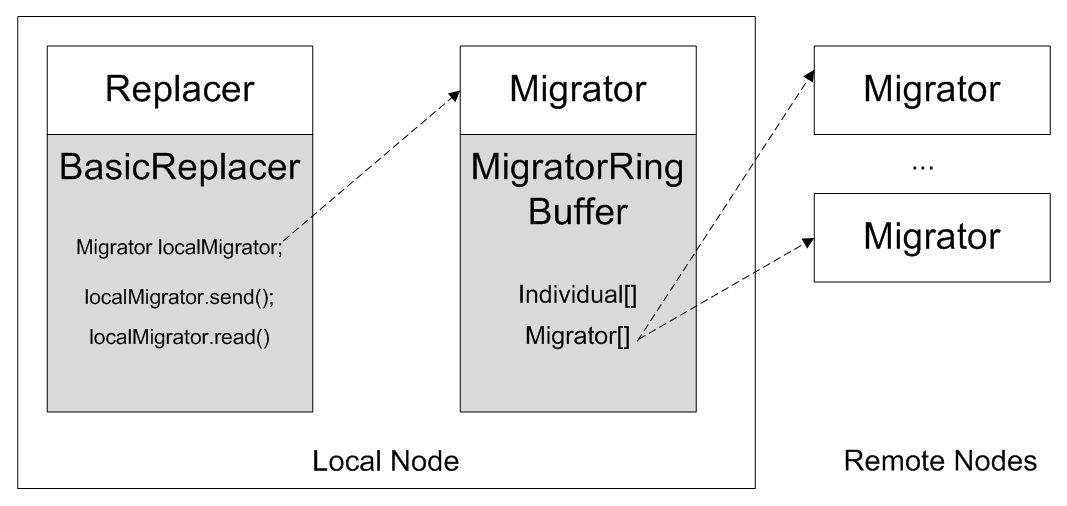
\includegraphics[scale=0.5]{images/migrator.eps}
\end{center} 
\caption{Utilizando el servicio {\em Migrator} para crear un AE distribuido basado en islas con topología en anillo (las cajas blancas son interfaces de los servicios y las grises son las implementaciones).} 
\label{MIGRATOR} 
\end{figure} 

% ¿ya se ha acabado? ¿Esto es todo? ¿Un manual de usuario? ¿No dices
% nada más? ¿Cuanto tiempo? ¿Cuantas líneas de código? ¿Algo? - JJ - FERGU: He dicho al principio cómo deben ser los servicios y he explicado los pasos para hacerlo con una tecnología.

\section{Conclusiones}
\label{sec:conclusions}
Este trabajo muestra los requisitos para crear un framework orientado a servicios para AEs y la tecnología escogida para cumplir esos requisitos.  Service Oriented Architecture (SOA) ofrece independencia del lenguaje, mecanismos de distribución o incluso sistemas operativos, permitiendo la integración de diferentes elementos. Sin embargo, algunos elementos deben considerarse en el desarrollo: los servicios son funciones de entrada/salida sin estado, los servicios pueden aparecer o desaparecer en tiempo real, y el orden de ejecución no debe estar fijo. En el campo de los AEs los servicios deben desarrollarse teniendo en cuenta estas restricciones. Este trabajo muestra el diseño abstracto de los elementos de un AE, junto con los requisitos tecnológicos a resolver. Se ha utilizado la tecnología OSGi como ejemplo. Los elementos para crear una SOA para AEs han sido presentados junto con un ejemplo de desarrollo.

Como trabajo futuro, se pretende realizar un estudio sobre escalabilidad utilizando otros algoritmos (como GRASP, Scatter Search, Ant Colony Optimization y otros). Además está planeado incrementar el uso de las ventajas de OSGi, como la administración de eventos o la gestión de servicios de forma más profunda. Finalmente, se plantea desarrollar un portal o un repositorio Maven\footnote{\url{http://www.maven.org}} para centralizar todas las implementaciones de problemas y algoritmos para permitir la distribución junto con la plataforma base. También se plantea un estudio sobre portar software existente (especialmente los frameworks escritos en Java, como DREAM o ECJ) a nuestro framework. Además, debido a la facilidad de enlazar implementaciones a interfaces, se plantea desarrollar la funcionalidad de elegir una u otra implementación dependiendo de varios parámetros, o por ejemplo, utilizar Programación Genética para evolucionar e hibridizar algoritmos.

\section*{Agradecimientos}



Este trabajo se está desarrollando gracias a la financiación del proyecto FEDER de la Unión Europea con título ``Sistema de Información y Predicción de bajo coste y autónomo para conocer el Estado de las Carreteras en tiempo real mediante dispositivos distribuidos'' (SIPEsCa) del Programa Operativo FEDER de Andalucía 2007-2013 y la beca FPU AP2009-2942 y los proyectos EvOrq (TIC-3903), CANUBE (CEI2013-P-14) y ANYSELF (TIN2011-28627-C04-02).
\begin{figure}
\begin{center} 

\epsfig{file=images/logos_SIPESCA_2.eps,width=5cm}
\end{center} 
%\caption{ } 
%\label{logos_SIPESCA_2} 
\end{figure}
\bibliographystyle{splncs}
\bibliography{osgiliath}

\end{document}

